\section{个性化联邦学习中的典型算法}
\addcontentsline{toe}{section}{{\currentchapter .2\ \ Existing Algorithms for Personalized Federated Learning}\numberline\,}
\label{sec:chap3-pfl-algo}

% NOT finished
% NOT indexed

本节主要介绍已有的一些基于正则化目标函数的个性化联邦学习算法,此类算法的基本形式见上一节\S~\ref{sec:chap3-pfl}~的式~\eqref{eq:pfl-general}。本报告称这一类的基于正则化目标函数的最优化问题为弱共识问题 (Weak Consensus Problem)\index{弱共识问题, Weak Consensus Problem}。本节将介绍一些基于此类问题而提出的个性化联邦学习算法。

\subsection*{无环随机梯度下降算法\texttt{L2SGD}}
% almost finished

这一类算法形式最简单的是文献\cite{hanzely2020federated}所引入的无环随机梯度下降 (Loopless Local SGD, L2SGD)\index{无环随机梯度下降, Loopless Local SGD, L2SGD} 算法\texttt{L2SGD}。其考虑的优化问题格式为
\begin{equation}
\label{eq:l2sgd}
\begin{array}{cl}
\minimize & F(\Theta) = f(\Theta) + \lambda \varphi(\Theta) \\
\text{where} & f(\Theta) = \frac{1}{K} \sum\limits_{k=1}^K f_i(\theta_i) \\
& \varphi(\Theta) = \frac{1}{2K} \sum\limits_{k=1}^K \left\lVert \theta_k - \bar{\theta} \right\rVert^2 = \frac{1}{2K} \sum\limits_{k=1}^K \left\lVert \theta_k - \frac{1}{K} \sum\limits_{j=1}^K \theta_j \right\rVert^2 \\
& \Theta = \col(\theta_1, \ldots, \theta_K).
\end{array}
\end{equation}
其中$\lambda \geqslant 0$是罚参数。当$0 < \lambda < \infty,$ 求解上述优化问题得到的模型$\bar{\theta}, \theta_1, \ldots, \theta_K$被称作是混合模型 (Mixed Models)。很容易看出,上述问题可以等价地转化为联邦临近算法\texttt{FedProx}所考察的问题~\eqref{eq:fedprox-whole}。

\begin{algorithm}[ht]
% \SetAlgoNoLine
% \DontPrintSemicolon
\SetKwInOut{Input}{Input}
\Input{xx}
{\bfseries Initiation:}\;
\caption{算法\texttt{L2SGD}\cite{hanzely2020federated}的伪代码}
\label{algo:l2sgd}
\end{algorithm}


文献\parencite{hanzely2020federated}定义问题~\ref{eq:l2sgd}目标函数$F(\Theta)$的随机梯度为
\begin{equation}
\label{eq:l2sgd-grad}
G(\Theta) := \begin{cases}
\frac{\nabla f(\Theta)}{1 - p}, & \text{概率$1-p$} \\
\frac{\lambda \nabla \varphi(\Theta)}{p}, & \text{概率$p$}
\end{cases}
\end{equation}
以上定义的随机梯度是是梯度$\nabla F$的无偏估计。这样的方法简化了$\nabla F$的计算,提高了整体算法的收敛率\cite{Kovalev2020_loopless}。值得特别注意的是,在随机梯度$G$的定义式~\eqref{eq:l2sgd-grad}~中,$\nabla f(\Theta) = \col(\nabla f_1(\theta_1), \cdots, \nabla f_K(\theta_K))$的计算是完全块分离的,在联邦学习的场景下,这一计算步骤只需要在子节点上执行计算,并不涉及与中心节点的通信,这对于以通信为主要瓶颈的联邦学习场景是巨大的优势。从这个意义上来说,无环随机梯度下降\texttt{L2SGD}也融入了跳步更新的思想。

文献\parencite{hanzely2020federated}对子节点上的目标函数做了进一步的假设,即假设$f_k$有有限和的结构
\begin{equation}
f_k(\theta_k) = \sum\limits_{j=1}^m f_{k, j}(\theta_k),
\end{equation}
并结合随机Kaczmarz方法 (Randomized Kaczmarz Method)\index{随机Kaczmarz方法, Randomized Kaczmarz Method}\cite{Strohmer_2008_Kaczmarz,Needell_2015_Kaczmarz} 或者说结合基于采样的随机梯度下降法 (SGD Algorithm with Importance Sampling)\cite{Needell_2015_Kaczmarz,Zhao2015_sampling},为问题~\eqref{eq:l2sgd}~的求解设计了所谓的无环随机梯度下降法,其伪代码见算法~\ref{algo:l2sgd}。实际上,随机梯度~\eqref{eq:l2sgd-grad}~也是基于采样的随机梯度。基于采样的随机梯度算法从收敛率到通信效率都有提升,是值得进一步研究的联邦学习优化算法。

\subsection*{\texttt{pFedMe}算法}
% almost finished

文献\parencite{t2020pfedme}考虑了与~\eqref{eq:l2sgd}~类似形式的问题
\begin{equation}
\label{eq:pfedme-one}
\minimize_{\theta,\theta_1,\ldots,\theta_K} \quad \sum\limits_{k=1}^K \left\{ f_k(\theta_k) + \frac{\lambda}{2} \left\lVert \theta_k - \theta \right\rVert^2 \right\}.
\end{equation}
特别地,文献\parencite{t2020pfedme}基于联邦学习中心节点--子节点这一二元结构,进一步将上述问题等价地转换为一个双层优化问题 (Bi-level Optimization Problem)\index{双层优化问题, Bi-level Optimization Problem}
\begin{equation}
\label{eq:pfedme-bilevel}
\begin{array}{cl}
\minimize & F(\theta) := \frac{1}{K} \sum\limits_{k=1}^K F_k(\theta), \\
\text{where} & F_k(\theta) = \min\limits_{\theta_k \in \R^d} \left\{ f_k(\theta_k) + \frac{\lambda}{2} \left\lVert \theta_k - \theta \right\rVert^2 \right\},
\end{array}
\end{equation}
相应求解算法\texttt{pFedMe}的伪代码见算法~\ref{algo:pfedme}。

\begin{algorithm}[ht]
% \SetAlgoNoLine
% \DontPrintSemicolon
{\bfseries Input:} $T, R, S, \lambda, \eta, \beta, \theta^{(0)} \in \R^d$\;
\For{each round $t = 0, \cdots, T-1$}{
    Server sends $\theta^{(t)}$ to all clients\;
    \For{each client $k = 1, \cdots, K$ in parallel}{
        $\theta_{k}^{(t, 0)} = \theta^{(t)}$\;
        \For{$r = 0,\cdots, R-1$}{
            Sample a mini-batch $b_r$\;
            find an approximate $\theta_k(\theta_{k}^{(t, r)})$ to the problem $\text{min} \{ \ell_k(\theta_k; b_r) + \frac{\lambda}{2} \left\lVert \theta_k - \theta_{k}^{(t, r)} \right\rVert^2 \}$\;
            Local update $\theta_{k}^{(t, r+1)} = \theta_{k}^{(t, r)} - \eta \lambda \left( \theta_{k}^{(t, r)} - \theta_k(\theta_{k}^{(t, r)}) \right)$\;
        }
        Server uniformly samples a subset of clients $\mathcal{S}^{(t)}$,\;
        each client in $\mathcal{S}^{(t)}$ sends the local $\theta_{k}^{(t, R)}$ to the server\;
    }
    Sever update $\theta^{(t+1)} = (1-\beta)\theta^{(t)} + \beta \sum \frac{\theta_{k}^{(t, R)}}{\# \mathcal{S}^t}$
}
\caption{\texttt{pFedMe}\cite{t2020pfedme}算法伪代码}
\label{algo:pfedme}
\end{algorithm}


很容易看到问题~\eqref{eq:pfedme-bilevel}~中的$F_k(\theta)$即为$f_k(\theta_k)$的Moreau包络~\eqref{eq:moreau_env}
\begin{equation*}
F_k(\theta) = \mathcal{M}_{f_k, \lambda} (\theta) := \inf\limits_{\theta_k} \left\{ f_k(\theta_k) + \frac{\lambda}{2} \lVert \theta_k - \theta \rVert^2 \right\}
\end{equation*}
相应最优化问题的解点即为临近算子
\begin{equation*}
\prox_{f_k, \lambda}: \theta \mapsto \argmin_{\theta_k} \left\{ f_k(\theta_k) + \frac{\lambda}{2} \lVert \theta_k - \theta \rVert^2 \right\}
\end{equation*}
在全局模型$\theta$处的取值。这个值即为算法\texttt{pFedMe}得到的子节点$k$上的个性化模型。算法\texttt{pFedMe}对双层优化~\eqref{eq:pfedme-bilevel}~的外层问题,即$F(\theta)$的优化求解采取的是随机梯度下降法。通过Moreau包络与临近算子的关系式~\eqref{eq:prox-moreau-relation}~可知双层优化问题~\eqref{eq:pfedme-bilevel}~的外层目标函数$F(\theta)$的梯度可以通过下式计算
\begin{equation}
\label{eq:pfedme-grad}
\nabla F(\theta) = \frac{1}{K} \sum\limits_{k=1}^K \nabla F_k(\theta) = \frac{1}{K} \sum\limits_{k=1}^K \nabla \mathcal{M}_{f_k, \lambda} (\theta) = \frac{1}{K} \sum\limits_{k=1}^K \lambda \left( \theta - \prox_{f_k, \lambda} (\theta) \right),
\end{equation}
相应的梯度下降的迭代格式为
\begin{equation}
\label{eq:pfedme-iter}
\begin{aligned}
\theta^{(t+1)} & = \theta^{(t)} - \eta \nabla F(\theta^{(t)}) = \theta^{(t)} - \eta \lambda \frac{1}{K} \sum\limits_{k=1}^K \left( \theta^{(t)} - \prox_{f_k, \lambda} (\theta^{(t)}) \right) \\
& = \frac{1}{K} \sum\limits_{k=1}^K \left( \theta^{(t)} - \eta \lambda \left( \theta^{(t)} - \prox_{f_k, \lambda} (\theta^{(t)}) \right) \right).
\end{aligned}
\end{equation}
以上格式可以分解为两部分,第一部分是在子节点上依次执行临近算子$\prox_{f_k, \lambda}$的求解
\begin{equation}
\label{eq:pfedme-prox-1}
\texttt{prox\_update}_k (\theta^{(t)}),
\end{equation}
以及全局模型的部分更新:
\begin{equation}
\label{eq:pfedme-local-1}
\theta^{(t)} - \eta \lambda \left( \theta^{(t)} - \prox_{f_k, \lambda} (\theta^{(t)}) \right).
\end{equation}
实际上,算法\texttt{pFedMe}的子节点上有全局模型$\theta^{(t)}$的一份拷贝$\omega_k^{(t,r)}$,这两个部分的更新实际上执行的是,利用全局模型的拷贝$\omega_k^{(t,r)}$更新个性化模型$\theta_k^{(t, r)}:$
\begin{equation}
\label{eq:pfedme-prox-2}
\theta_k^{(t, r)} \gets \texttt{prox\_update}_k (\omega_{k}^{(t, r)}; b_r)
\end{equation}
以及$\omega_k^{(t,r)}$自身的更新:
\begin{equation}
\label{eq:pfedme-local-2}
\omega_k^{(t,r+1)} \gets \omega_k^{(t,r)} - \eta \lambda \left( \omega_k^{(t,r)} - \prox_{f_k, \lambda} (\omega_k^{(t,r)}) \right).
\end{equation}
第二部分是子节点模型在中心节点上的聚合:
\begin{equation}
\label{eq:pfedme-avg}
\theta^{(t+1)} \gets (1-\beta)\theta^{(t)} + \frac{\beta}{\# \mathcal{S}^{(t)}} \sum\limits_{k \in \mathcal{S}^{(t)}} \omega_{k}^{(t, R)}.
\end{equation}
算法\texttt{pFedMe}整个迭代循环值得特别注意的是,以上分解的两部分并不是交替进行的,而是在子节点上执行一定步数($R$步)的第一部分的迭代之后,才进行与中心节点的通信,在中心节点上执行第二部分的聚合。这是另一种形式的跳步更新的方法。

\subsection*{\texttt{Ditto}算法}
% almost finished

文献\parencite{li_2021_ditto}进一步发展了联邦临近算法\texttt{FedProx}\cite{sahu2018fedprox}添加临近项求解子问题的思想,将子节点的优化问题~\eqref{eq:fedprox}~改进为一个双层优化问题
\begin{equation}
\label{eq:ditto-bilevel}
\begin{array}{cl}
\minimize\limits_{\omega_k} & h_k(\omega_k, \theta^*) := f_k(\omega_k) + \frac{\mu}{2} \lVert \omega_k - \theta^* \rVert^2, \\
\text{subject to} & \theta^* \in \argmin\limits_{\theta} G(f_1(\theta), \cdots, f_K(\theta)),
\end{array}
\end{equation}
其中$G$是中心节点上执行子节点模型参数聚合的函数,例如\texttt{FedAvg}算法中采用的求均值函数。这一问题格式是以子节点为主视角的格式,是第一批\footnote{稍早提出的自适应个性化联邦学习算法\texttt{APFL}\cite{deng2020_apfl}~\ref{algo:apfl}~也采用了类似的视角}明确基于这一视角的个性化联邦学习建模、求解方法。基于这一问题格式,文献\parencite{li_2021_ditto}设计了\texttt{Ditto}算法进行优化求解,其伪代码见算法~\ref{algo:ditto}。

\begin{algorithm}[ht]
% \SetAlgoNoLine
% \DontPrintSemicolon
\SetKwInOut{Input}{Input}
\Input{penalty coeffecient $\mu,$ learning rate $\eta,$ methods $\operatorname{\mathbf{UpdateGlobal}}, \operatorname{\mathbf{Aggregate}}$}
{\bfseries Initiation:}\;
\Indp
    {\bfseries Init server:} global model parameters $\theta^{(0)} \in \R^d$\;
    {\bfseries Init clients:} local model parameters $\omega_k^{(0)} \in \R^d, ~ \forall k \in [K]$\;
\Indm
\For{each round $t = 0, 1, \cdots, T-1$}{
    $\mathcal{S}^{(t)} \gets$ (random set of clients) $\subseteq [K]$\;
    broadcast $\theta^{(t)}$ to clients $k \in \mathcal{S}^{(t)}$\;
    \For{each client $k \in \mathcal{S}^{(t)}$ {\bfseries in parallel}}{
        \tcc{solve the local sub-problem of $G(\dot)$ inexactly starting from $\theta^{(t)}$ to obtain $\theta_k^{(t)}$}
        $\theta_k^{(t)} \gets \operatorname{\mathbf{UpdateGlobal}}(\theta^{(t)}, f_k)$\;
        \tcc{update the personalized model via solving \eqref{eq:ditto-local}}
        $\omega_k^{(t+1)} \gets \omega_k^{(t)} - \eta \left( \nabla f_k(\omega_k^{(t)}) + \mu (\omega_k^{(t)} - \theta^{(t)}) \right)$\;
        send $\Delta_k^{(t)} \gets \theta_k^{(t)} - \theta^{(t)}$ to server\;
    }
    {\bfseries Server Update:}\;
    \Indp
    $\theta^{(t+1)} \gets \operatorname{\mathbf{Aggregate}} (\theta^{(t)}, \{ \Delta_k^{(t)} \}_{k \in \mathcal{S}^{(t)}})$\;
    \Indm
}
\caption{算法\texttt{Ditto}\cite{li_2021_ditto}的伪代码}
\label{algo:ditto}
\end{algorithm}


可以看到,文献\parencite{li_2021_ditto}考虑的双层优化问题~\eqref{eq:ditto-bilevel}~的内层问题实际上可以视作一个独立的联邦优化问题,只对全局模型参数进行优化求解;外层问题实际上只涉及了子节点上求解临近算子的问题。如果以中心节点为主视角,那么问题~\eqref{eq:ditto-bilevel}~实际上就是联邦平均算法\texttt{FedAvg}考虑的问题~\eqref{eq:fedavg-constraint},同时在每个子节点上附带一个求解临近算子的问题达到模型个性化的目的。这个个性化的模型并不参与全局模型的更新。这样,全局模型与个性化模型被解耦合,迭代更新可以更灵活地进行。

类似于\texttt{pFedMe}算法~\ref{algo:pfedme},\texttt{Ditto}算法~\ref{algo:ditto}~的子节点实际要执行2个优化问题的求解,即全局模型的更新 (双层优化问题~\eqref{eq:ditto-bilevel}~内层问题的求解)
\begin{equation}
\label{eq:ditto-global}
\theta_k^{(t)} \gets \operatorname{\mathbf{UpdateGlobal}}(\theta^{(t)}, f_k),
\end{equation}
以及临近算子的求解 (双层优化问题~\eqref{eq:ditto-bilevel}~外层问题的求解)
\begin{equation}
\label{eq:ditto-local-1}
\omega_k^{(t+1)} \gets \prox_{f_k, \mu} (\theta^{(t)}) = \argmin\limits_{\omega_k} \left\{ f_k(\omega_k) + \frac{\mu}{2} \lVert \omega_k - \theta^{(t)} \rVert^2 \right\}.
\end{equation}
与本报告之前介绍的算法 (\texttt{FedSplit}算法~\ref{algo:fedsplit}、\texttt{pFedMe}算法~\ref{algo:pfedme}~等) 不同之处在于,\texttt{Ditto}算法在每次循环对以上问题的求解只执行一步 (随机) 梯度下降
\begin{equation}
\label{eq:ditto-local-2}
\omega_k^{(t+1)} \gets \omega_k^{(t)} - \eta \left( \nabla f_k(\omega_k^{(t)}) + \mu (\omega_k^{(t)} - \theta^{(t)}) \right),
\end{equation}
这样以伴随全局模型的更新而不断修正临近算子的中心项$\theta^{(t)},$ 而完成双层优化问题~\eqref{eq:ditto-bilevel}~外层问题的求解。这是自然的,因为这部分更新是双层优化问题的外层问题的迭代更新,而\texttt{FedSplit}算法、\texttt{pFedMe}算法相应的则是内循环以及内层问题的更新。

\subsection*{自适应个性化联邦学习算法\texttt{APFL}}
% almost finished

比\parencite{li_2021_ditto}稍早的文献\parencite{deng2020_apfl}也考虑了类似~\eqref{eq:ditto-bilevel}~的双层优化问题
\begin{equation}
\label{eq:apfl-bilevel}
\begin{array}{cl}
\minimize\limits_{\omega_k \in \dom f_k} & h_k(\omega_k, \theta^*) := f_k( \alpha_k \omega_k + (1 - \alpha_k) \theta^* ), \\
\text{subject to} & \theta^* \in \argmin\limits_{\theta} \frac{1}{K} \sum\limits_{k=1}^K (f_1(\theta) + \cdots + f_K(\theta)),
\end{array}
\end{equation}
其中$\alpha_k \in (0, 1)$被称作是混合权重 (Mixture Weights)。文献\parencite{deng2020_apfl}针对这一双层优化问题~\eqref{eq:apfl-bilevel}~基于随机梯度下降方法提出了自适应个性化联邦学习算法\texttt{APFL},其伪代码可见算法~\ref{algo:apfl}。

\begin{algorithm}[!htb]
% \SetAlgoNoLine
% \DontPrintSemicolon
\SetKwInOut{Input}{Input}
\Input{mixture weights $\alpha_1, \ldots, \alpha_K,$ synchronization gap $\tau$}
{\bfseries Initiation:}\;
\Indp
    {\bfseries Init server:} global model parameters $\theta^{(0)} \in \R^d,$ random set of clients $S^{(t)} \subseteq [K]$\;
    {\bfseries Init clients:} local model parameters $\omega_k^{(0)} \in \R^d, ~ \theta_k^{(0)} \gets \theta^{(0)}, ~ \forall k \in [K]$\;
    {\bfseries Constants:} condition number $\kappa \gets \frac{L}{\mu},$ $a \gets \max\{128\kappa, \tau\}$\;
\Indm
\For{each round $t = 0, 1, \cdots, T-1$}{
    \For{each client $k \in \mathcal{S}^{(t)}$ {\bfseries in parallel}}{
        $\bar{\omega}_k^{(t)} \gets \alpha_k \omega_k^{(t)} + (1-\alpha_k) \theta_k^{(t)}$ \tcc*[h]{mixture model}\;
        $\eta^{(t)} \gets \frac{16}{\mu(t+a)}$ \tcc*[h]{decay learning rate}\;
        $\theta_k^{(t+1)} \gets \theta_k^{(t)} - \eta^{(t)} \nabla f_k(\theta_k^{(t)})$ \tcc*[h]{inner problem (global model) update}\;
        $\omega_k^{(t+1)} \gets \omega_k^{(t)} - \eta^{(t)} \nabla f_k(\bar{\omega}_k^{(t)})$ \tcc*[h]{outer problem (personalized model) update}\;
        \tcc{Optional: adaptive mixture weights update}
        \tcc{$\alpha_k \gets \alpha_k - \eta^{(t)} \nabla_{\alpha_k} f_k(\bar{\omega}_k^{(t)}) = \alpha_k - \eta^{(t)} \left\langle \omega_k^{(t)} - \theta_k^{(t)}, \nabla f_k(\bar{\omega}_k^{(t)}) \right\rangle$}
    }
    \uIf{$t$ not divides synchronization gap $\tau$}{
        {\bfseries Server updates}: $\mathcal{S}^{(t+1)} \gets \mathcal{S}^{(t)}$\;
    }
    \Else{
        each client $k \in \mathcal{S}^{(t)}$ sends $\theta_k^{(t+1)}$ to server\;
        {\bfseries Server updates}:\;
        \Indp
        $\theta^{(t+1)} \gets \frac{1}{\# \mathcal{S}^{(t)}} \theta_k^{(t+1)}$\;
        $\mathcal{S}^{(t+1)} \gets$ (random set of clients) $\subseteq [K]$\;
        broadcast $\theta^{(t+1)}$ to clients $k \in S^{(t+1)}:$ $\theta_k^{(t+1)} \gets \theta^{(t+1)}$\;
        \Indm
    }
final personalized model: $\hat{\omega}_k \gets \frac{1}{S_T}\sum\limits_{t=1}^{T} p_t \left( \alpha_k \omega_k^{(t)} + (1-\alpha_k)\frac{1}{\#\mathcal{S}^{(t-1)}}\sum\limits_{k\in\mathcal{S}^{(t-1)}}\theta_k^{(t)} \right)$\;
final global model: $\hat{\theta} \gets \frac{1}{S_T}\sum\limits_{t=1}^{T} \frac{p_t}{\#\mathcal{S}^{(t-1)}} \sum\limits_{k\in\mathcal{S}^{(t-1)}}\theta_k^{(t)}$\;
where $p_t = (t+a)^2, S_T = \sum\limits_{t=1}^{T}p_t$\;
}
\caption{算法\texttt{APFL}\cite{deng2020_apfl}的伪代码}
\label{algo:apfl}
\end{algorithm}


可以看到,与问题格式~\eqref{eq:ditto-bilevel}~最主要的区别是,\eqref{eq:apfl-bilevel}的外层问题对应的模型个性化的方法,采用了辅助模型参数$\omega_k$与全局模型$\theta^*$的凸组合$\alpha_k \omega_k + (1 - \alpha_k) \theta^*,$ 而不是临近项$\frac{\mu}{2} \lVert \omega_k - \theta^* \rVert^2$的的形式;而混合权重$\alpha_k$起到临近项中罚参数$\mu$类似的调节子节点上模型个性化程度的作用。最终得到的个性化模型为
\begin{equation}
\label{eq:apfl-per-model}
\begin{array}{cl}
& \hat{\omega}_k = \alpha_k \omega_k^* + (1 - \alpha_k) \theta^*, \\
\text{其中} & \omega_k^* = \argmin\limits_{\omega_k \in \dom f_k} f_k( \alpha_k \omega_k + (1 - \alpha_k) \theta^* ).
\end{array}
\end{equation}

值得特别注意的是,当$\dom f_k$是全空间$\R^d$的一个真子集时,通过式~\eqref{eq:apfl-per-model}个性化模型$\hat{\omega}_k$可能并非目标函数$f_k$的极小点。具体如图~\ref{fig:apfl}~所示,当取$\alpha_k = \frac{1}{2},$ 同时假设$\dom f_k,$ 即$\omega_k$的搜索区域是图中浅灰色阴影区域时,凸组合
\begin{equation*}
\alpha_k \omega_k^* + (1 - \alpha_k) \theta^*
\end{equation*}
能取到的区域实际上是图中深灰色区域。可以看到深灰色区域并不包含$f_k$的极小点。当$\omega_k$的搜索区域变大,变成图~\ref{fig:apfl}~中的区域$\widetilde{\dom f_k}$时,通过迭代搜索得到的$\omega_k^*$才能使得$\hat{\omega}_k$成为$f_k$的极小点。但是在这种情况下,$\hat{\omega}_k$完全可以脱离整个联邦学习的训练网络,通过直接极小化$f_k$ (即只使用节点$k$上自身的数据进行训练) 获取,这与个性化联邦学习算法的目的是相违背的。

\begin{figure}[H]
\centering
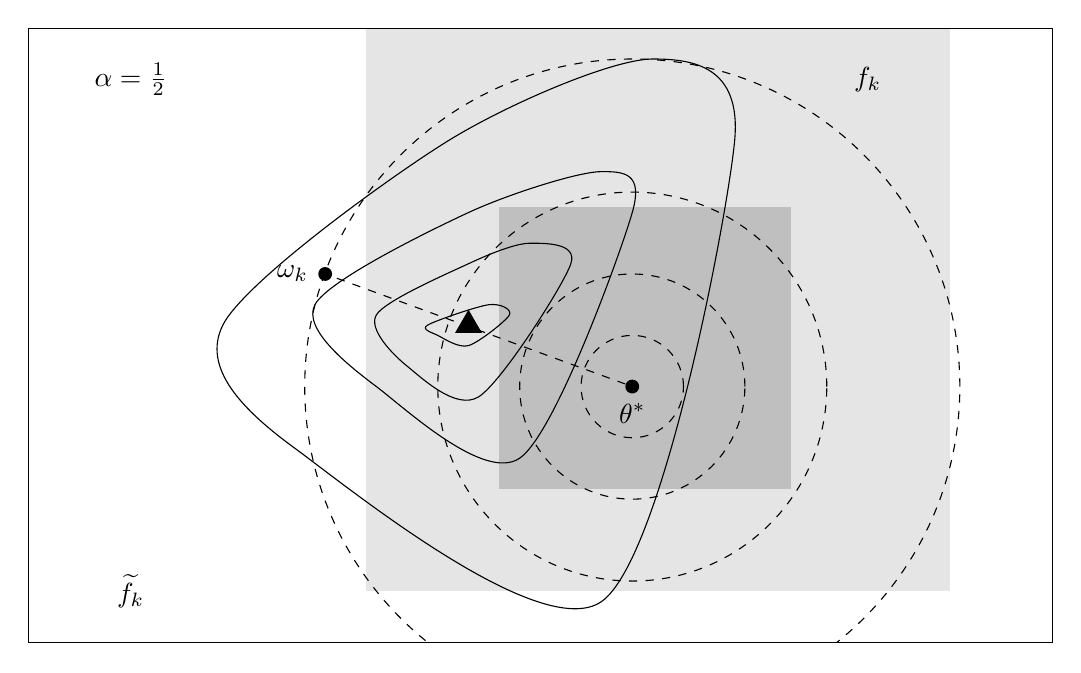
\begin{tikzpicture}[scale=1.3]
% \coordinate (origin) at (0, 0);
\coordinate (rect1) at (-5, -3);
\coordinate (rect2) at (5, 3);
\fill [gray!20] (-1.7, -2.5) rectangle (4, 3);
\fill [gray!50] (-0.4, -1.5) rectangle (2.45, 1.25);
\draw (rect1) rectangle (rect2);
\node at (3.2, 2.5) {$\dom f_k$};
\node at (-4, -2.5) {$\widetilde{\dom f_k}$};
\node at (-4, 2.5) {$\alpha = \frac{1}{2}$};
\draw[] plot [smooth cycle] coordinates {(-1, 0) (-0.7, -0.1) (-0.3, 0.2) (-0.5, 0.3) (-1.1, 0.1)};
\draw[] plot [smooth cycle] coordinates {(-1.3, -0.3) (-0.6, -0.6) (0.3, 0.7) (-0.1, 0.9) (-0.7, 0.7) (-1.6, 0.2)};
\draw[] plot [smooth cycle] coordinates {(-1.6, -0.5) (-0.2, -1.2) (0.9, 1.2) (0.6, 1.6) (-0.7, 1.2) (-2.2, 0.3)};
\draw[] plot [smooth cycle] coordinates {(-2.4, -1.1) (0.6, -2.6) (1.9, 1.9) (1.1, 2.7) (-0.9, 1.9) (-3.1, 0.1)};
\node at (0.9, -0.5) (theta) [circle, fill=black, inner sep=0pt, minimum size=5pt, label=below:{$\theta^*$}] {};
\node at (-2.1, 0.6) (omega1) [circle, fill=black, inner sep=0pt, minimum size=5pt, label=left:{$\omega_k$}] {};
\draw[dashed, thin] (theta) -- (omega1);
\draw plot[only marks, mark=triangle*, mark size=4pt, thick] coordinates {(-0.7, 0.1)};
\begin{scope}
\clip (rect1) rectangle (rect2);
\draw[dashed, thin] (theta) circle (0.5);
\draw[dashed, thin] (theta) circle (1.1);
\draw[dashed, thin] (theta) circle (1.9);
\draw[dashed, thin] (theta) circle (3.2);
\end{scope}
\end{tikzpicture}
\caption{$f_k(\alpha_k \omega_k + (1 - \alpha_k) \theta^*)$的示意图}
\label{fig:apfl}
\end{figure}


\subsection*{动态正则化联邦学习算法\texttt{FedDyn}}
% almost finished

本节已经介绍的算法,包括在\S~\ref{sec:chap2-ppa}~中介绍的联邦临近算法\texttt{FedProx},都是以添加某种形式的临近项作为子节点目标函数的正则化项,以此达到某种意义上的模型个性化的目的。例如联邦临近算法\texttt{FedProx},在算法迭代更新第$t+1$轮,每个子节点优化的目标函数为如下的带临近项的函数~\eqref{eq:fedprox}
\begin{equation*}
f_k(\theta_k) + \frac{\mu}{2} \lVert \theta_k - \theta^{(t)} \rVert^2
\end{equation*}
文献\parencite{acar2021feddyn}对此进行了进一步的改进,提出了所谓的动态正则化的目标函数
\begin{equation}
\label{eq:feddyn}
F_k(\theta_k) := f_k(\theta_k) - \langle \nabla f_k(\theta_k^{(t)}), \theta_k \rangle + \frac{\mu}{2} \lVert \theta_k - \theta^{(t)} \rVert^2.
\end{equation}
为求解这一优化问题,文献\parencite{acar2021feddyn}设计了动态正则化联邦学习算法 (Federated Dynamic Regularizer) \texttt{FedDyn},其伪代码见算法~\ref{algo:feddyn}。

\begin{algorithm}[ht]
% \SetAlgoNoLine
% \DontPrintSemicolon
\SetKwInOut{Input}{Input}
\Input{penalty coeffecient $\mu$}
{\bfseries Initiation:}\;
\Indp
    {\bfseries Init server:} global model parameters $\theta^{(0)} \in \R^d,$ $h = 0 \in \R^d$\;
    {\bfseries Init clients:} local gradient $\mathfrak{g}_k^{(0)} \gets 0 \in \R^d, ~ \forall k \in [K]$\;
\Indm
\For{each round $t = 0, 1, \cdots, T-1$}{
    $S^{(t)} \gets$ (random set of clients) $\subseteq [K]$\;
    broadcast $\theta^{(t)}$ to clients $k \in S^{(t)}$\;
    \For{each client $k \in \mathcal{S}^{(t)}$ {\bfseries in parallel}}{
        $\theta_k^{(t+1)} \gets \argmin\limits_{\theta_k} \left\{ f_k(\theta_k) - \langle \mathfrak{g}_k^{(t)}, \theta_k \rangle + \frac{\mu}{2} \lVert \theta_k - \theta^{(t)} \rVert^2 \right\}$ \;
        $\mathfrak{g}_k^{(t+1)} \gets \mathfrak{g}_k^{(t)} - \mu (\theta_k^{(t+1)} - \theta^{(t)})$\;
        send $\theta_k^{(t+1)}$ to server\;
    }
    {\bfseries Server Update:}\;
    \Indp
    $h^{(t+1)} \gets h^{(t)} - \frac{1}{\mu} \left(\sum\limits_{k \in S^{(t)}} \theta_k^{(t+1)} - \theta^{(t)} \right)$\;
    $\theta^{(t+1)} \gets \left( \frac{1}{\# S^{(t)}}\sum\limits_{k \in S^{(t)}} \theta_k^{(t+1)} \right) - \frac{1}{\mu} h^{(t+1)}$\;
}
\caption{算法\texttt{FedDyn}\cite{acar2021feddyn}的伪代码}
\label{algo:feddyn}
\end{algorithm}


可以看到,所谓的动态正则化~\eqref{eq:feddyn},指的是在原有的临近正则项$\frac{\mu}{2} \lVert \theta_k - \theta^{(t)} \rVert^2$的基础上减去了自变量$\theta_k$与上一步的$\theta_k^{(t-1)}$处的梯度的内积$\langle \nabla f_k(\theta_k^{(t)}), \theta_k \rangle.$ 实际上,子节点$k$上的目标函数$F_k(\theta_k)$可以等价地调整为
\begin{equation}
\label{eq:feddyn-adjusted}
\begin{aligned}
F_k(\theta_k) & = f_k(\theta_k) - \langle \nabla f_k(\theta_k^{(t)}), \theta_k - \theta_k^{(t)} \rangle + \frac{\mu}{2} \lVert \theta_k - \theta^{(t)} \rVert^2 \\
& = \left( f_k(\theta_k) + \frac{\mu}{2} \lVert \theta_k - \theta^{(t)} \rVert^2 \right) - \langle \nabla f_k(\theta_k^{(t)}), \theta_k - \theta_k^{(t)} \rangle.
\end{aligned}
\end{equation}
对以上目标函数进行迭代求解的每一步 (第$t+1$步),相当于利用$f_k$在上一步迭代点$\theta_k^{(t)}$处的梯度方向
\begin{equation*}\mathfrak{g}_k^{(t)} := \nabla f_k(\theta_k^{(t)}),
\end{equation*}
对带临近正则项的函数
\begin{equation*}
f_k(\theta_k) + \frac{\mu}{2} \lVert \theta_k - \theta^{(t)} \rVert^2
\end{equation*}
的下降方向进行修正,如图~\ref{fig:feddyn}~所示。

\begin{figure}[H]
\centering
\begin{tikzpicture}[scale=1.6]
% \coordinate (origin) at (0, 0);
\draw (-4, -3) rectangle (5, 3);
\node at (-3,-2.5) {$\dom f_k$};
\draw[] plot [smooth cycle] coordinates {(-1, 0) (-0.7, -0.1) (-0.3, 0.2) (-0.5, 0.3) (-1.1, 0.1)};
% \draw[] plot [smooth cycle] coordinates {(-1.3, -0.3) (-0.6, -0.6) (0.3, 0.7) (-0.1, 0.9) (-0.7, 0.7) (-1.6, 0.2)};
\draw[] plot [smooth cycle] coordinates {(-1.6, -0.5) (-0.2, -1.2) (0.9, 1.2) (0.6, 1.6) (-0.7, 1.2) (-2.2, 0.3)};
\draw[] plot [smooth cycle] coordinates {(-2.4, -1.1) (0.6, -2.6) (1.9, 1.9) (1.1, 2.7) (-0.9, 1.9) (-3.1, 0.1)};
\node at (0.9, -0.5) (global) [circle, fill=black, inner sep=0pt ,minimum size=5pt, label=below:{$\theta^{(t)}$}] {};
\node at (1.2, 0.5) (local) [circle, fill=black, inner sep=0pt, minimum size=5pt, label=above:{$\theta_k^{(t)}$}] {};
\coordinate (min1) at (-0.7, 0.1);
\draw plot[only marks, mark=triangle*, mark size=4pt, thick] coordinates {(min1)};
\coordinate (min2) at (0.1, -0.6);
\draw plot[only marks, mark=star, mark size=4pt, thick] coordinates {(min2)};
\path (local) edge [draw, dashed, -{Stealth}] ($(local)!0.4!(min1)$);
\path (local) edge [draw, dashed, -{Stealth}] ($(local)!0.5!(min2)$);
\node at (0.6, 0.1) (next) [circle, fill=black, inner sep=0pt, minimum size=5pt, label=left:{$\theta_k^{(t+1)}$}] {};
\path (local) edge [draw, -{Stealth}] (next);
\begin{scope}
\clip (-4, -3) rectangle (5, 3);
\draw[dashed, thin] (global) circle (0.5);
% \draw[dashed, thin] (global) circle (1.1);
\draw[dashed, thin] (global) circle (1.9);
\draw[dashed, thin] (global) circle (3.2);
\end{scope}
\end{tikzpicture}
\caption{动态正则化联邦学习算法\texttt{FedDyn}子节点模型参数更新示意图}
\label{fig:feddyn}
\end{figure}


动态正则化问题~\eqref{eq:feddyn}~另一个值得注意的地方是,它的一阶最优性条件是
\begin{equation}
\label{eq:feddyn-opt-cond}
\nabla f_k(\theta_k^{(t+1)}) - \nabla f_k(\theta_k^{(t)}) + \mu \left( \theta_k^{(t+1)} - \theta^{(t)} \right),
\end{equation}
那么,子节点$k$上的局部梯度值序列
\begin{equation*}
\mathfrak{g}_k^{(t)} = \nabla f_k(\theta_k^{(t)}), ~ t = 0, 1, \ldots, T
\end{equation*}
即可以通过如下的方式迭代更新
\begin{equation}
\label{eq:feddyn-grad-iter}
\mathfrak{g}_k^{(t+1)} \gets \mathfrak{g}_k^{(t)} - \mu (\theta_k^{(t+1)} - \theta^{(t)}).
\end{equation}
这对于计算以及算法的实现是巨大的便利。

% \begin{equation}
% \label{eq:fedu}
% \minimize \quad \sum\limits_{k=1}^K f_k(x_k) + \dfrac{\lambda}{2} \sum\limits_{k=1}^K \sum\limits_{j\in\mathcal{N}_k} \lVert \theta_k - \theta_j \rVert^2
% \end{equation}

\subsection*{\texttt{pFedMac}算法}
% almost finished

动态正则化联邦学习算法\texttt{FedDyn}本质上是通过了使用某些特定的方向对个性化模型参数的迭代更新进行修正。有类似做法的是文献\parencite{li2021pfedmac}。其考虑的是如下的双层优化问题
\begin{equation}
\label{eq:pfedmac}
\begin{array}{cl}
\minimize & F(\theta) = \frac{1}{K} \sum\limits_{k=1}^K F_k(\theta), \\
\text{where} & F_k(\theta) := \min\limits_{\theta_k} \left\{ f_k(\theta_k) - \mu \langle \theta_k, \theta \rangle + \frac{\mu}{2} \lVert \theta \rVert^2_2 \right\}.
\end{array}
\end{equation}
实际上,可以进一步写为
\begin{equation}
\label{eq:pfedmac-adjusted}
\begin{array}{cl}
\minimize & F(\theta) = \frac{1}{K} \sum\limits_{k=1}^K F_k'(\theta) + \frac{\mu}{2} \lVert \theta \rVert^2_2, \\
\text{where} & F_k'(\theta) := \min\limits_{\theta_k} \left\{ f_k(\theta_k) - \mu \langle \theta_k, \theta \rangle \right\}.
\end{array}
\end{equation}
可以看到以上格式利用了全局模型参数$\theta,$ 对个性化模型参数$\theta_k$进行了修正;同时,外层问题的目标函数添加了自变量$\theta$的$\ell_2$-正则项。在概率与统计中,$\langle \theta_k, \theta \rangle$可解释为个性化模型$\theta_k$与全局模型$\theta$的相关性,因此~\eqref{eq:pfedmac}~对子节点目标函数的改进技术被称作是极大化 (全局模型与个性化模型) 相关性 (Maximizing Correlation)的技术,相应的求解算法被称作是极大化相关性算法 (Personalized Federated Learning via Maximizing
Correlation) \texttt{pFedMac},其伪代码可见算法~\ref{algo:pfedmac}。

\begin{algorithm}[ht]
% \SetAlgoNoLine
% \DontPrintSemicolon
\SetKwInOut{Input}{Input}
\Input{learning rate $\eta$, penalty coefficient $\lambda$, $\beta$}
% {\bfseries Server executes:}\;
% \Indp
{\bfseries Initiation:} global (server) model parameters $\theta^{(0)} \in \R^d$\;
\For{each round $t = 0, 1, \cdots, T-1$}{
    $\mathcal{S}^{(t)} \gets$ (random set of clients) $\subseteq [K]$\;
    broadcast $\theta^{(t)}$ to clients $k \in \mathcal{S}^{(t)}$\;
    \For{each client $k \in \mathcal{S}^{(t)}$ {\bfseries in parallel}}{
        $\theta_k^{(t)} \gets$ {\bfseries ClientUpdate}$(k, \theta^{(t)})$\;
        send $\theta_k^{(t)}$ to server\;
    }
    {\bfseries Server Update:}\;
    \Indp
    $\theta^{(t+1)} \gets (1 - \beta) \theta^{(t)} + \frac{\beta}{\lvert \mathcal{S}^{(t)} \rvert} \sum\limits_{k\in \mathcal{S}^{(t)}} \theta_k^{(t)}$\;
    \Indm
}
% \Indm
\vspace{0.2em}
{\bfseries ClientUpdate}$(k, \theta)$: \tcc*[h]{on client $k$}\;
\Indp
$\omega_k^{(t,0)} = \theta_k^{(t,0)} = \theta^{(t)}$\;
\For{local step $r = 0, 1, \cdots, R-1$}{
    $\mathcal{D}_{k, r} \gets$ (sample a mini-batch data)\;
    $\omega_k^{(t,r)} \gets \argmin_{\omega_k} \left\{ \ell_k(\omega_k; \mathcal{D}_{k, r}) - \lambda \langle \omega_k, \theta_k^{(t,r)} \rangle \right\}$\;
    $\theta_k^{(t,r+1)} \gets \theta_k^{(t,r)} - \eta\lambda \left( \theta_k^{(t,r)} - \omega_k^{(t,r)} \right)$\;
}
\Return{$\theta_k^{(t,R)}$}
\caption{算法\texttt{pFedMac}\cite{li2021pfedmac}的伪代码}
\label{algo:pfedmac}
\end{algorithm}


另一方面,可以观察到双层优化问题~\eqref{eq:pfedmac}~可以有如下的变形
\begin{equation*}
\begin{aligned}
F_k(\theta) & = \min\limits_{\theta_k} \left\{ f_k(\theta_k) - \mu \langle \theta_k, \theta \rangle + \frac{\mu}{2} \lVert \theta \rVert^2_2 \right\} \\
& = \min\limits_{\theta_k} \left\{ f_k(\theta_k) + \frac{\mu}{2} \lVert \theta_k - \theta \rVert^2_2 - \frac{\mu}{2} \lVert \theta_k \rVert^2_2 \right\} \\
& = \min\limits_{\theta_k} \left\{ f_k(\theta_k) + \frac{\mu}{2} \lVert \theta_k - \theta \rVert^2_2 - \frac{\mu}{2} \langle \theta_k, \theta_k \rangle \right\}.
\end{aligned}
\end{equation*}
这一形式可以与动态正则化联邦学习算法\texttt{FedDyn}的子节点问题格式~\eqref{eq:feddyn}~(或者~\eqref{eq:feddyn-adjusted})形成类比。也就是说,我们可以设计算法,在$t+1$步进行求解内层的问题时,利用上一步迭代点$\theta_k^{(t)}$的方向对带临近正则项的函数
\begin{equation*}
f_k(\theta_k) + \frac{\mu}{2} \lVert \theta_k - \theta^{(t)} \rVert^2
\end{equation*}
的下降方向进行修正。

文献\parencite{li2021pfedmac}另外的贡献是,考察了稀疏 (Sparse) 个性化模型的问题
\begin{equation}
\label{eq:pfedmac-sparse}
\begin{array}{cl}
\minimize & F(\theta) = \frac{1}{K} \sum\limits_{k=1}^K F_i(\theta), \\
\text{where} & F_k(\theta) := \min\limits_{\theta_k} \left\{ f_k(\theta_k) - \mu \langle \theta_k, \theta \rangle + \frac{\mu}{2} \lVert \theta \rVert^2_2 + \gamma \lVert \theta_k \rVert_1 \right\}
\end{array}
\end{equation}
以及对联邦学习中心节点--子节点这一二元结构的进一步扩展,即利用中心节点--次中心节点\footnote{一般称作边缘节点 (Edge)\cite{Liu_2020_Hierarchical} 或者枢纽 (Hub)\cite{proxskip-vr}}--子节点的三层结构\cite{Liu_2020_Hierarchical}来实现个性化联邦学习。具体来说,子节点以一定方式 (例如按地域分布) 形成一些集群 (Cluster),每一个集群有一个次中心节点,用于聚合该集群内的子节点模型参数
\begin{equation*}
\theta_{k,1}, \ldots, \theta_{k, J_k},
\end{equation*}
并与中心节点通信。相应的模型可以写为
\begin{equation}
\label{eq:pfedmac-sh}
\begin{array}{cl}
\minimize & F(\theta) = \frac{1}{K} \sum\limits_{k=1}^K F_i(\theta), \\
\text{where} & F_k(\theta) := \min\limits_{\theta_k} \left\{ \frac{1}{J_k} \sum\limits_{j=1}^{J_k} F_{k, j} (\theta_k) - \mu_2 \langle \theta_k, \theta \rangle + \frac{\mu_2}{2} \lVert \theta \rVert^2_2 \right\} \\
& F_{k, j}(\theta_k) := \min\limits_{\theta_{k, j}} \left\{ f_{k, j} (\theta_{k, j}) - \mu_2 \langle \theta_{k, j}, \theta_k \rangle + \frac{\mu_2}{2} \lVert \theta_k \rVert^2_2 + \gamma \lVert \theta_{k, j} \rVert_1 \right\}.
\end{array}
\end{equation}
随着联邦学习网络规模的扩大,类似的分层次的 (Hierarchical) 联邦学习结构的应用会越来越普遍。相应地,结合子节点聚类的联邦学习算法也越来越受到关注\cite{Sattler_2021_cfl, Ghosh_2022_cfl, fl_fpfc_2022, Zhang_2023_fedmds}。
